%%%%%%%%%%%%%%%%%%%%%%%%%%%%%%%%%
%
%       EXERCÍCIO
%
%%%%%%%%%%%%%%%%%%%%%%%%%%%%%%%%%

\ifdefstring{\atividade}{prova}{%
    \ifdefstring{\modo}{objetivo}{%
        \renewcommand{\valorquestao}{\ValorQObj\ ponto}
    }{%
        \renewcommand{\valorquestao}{\ValorQDisc\ pontos}
    }%
}%

\begin{exercicioBanco}[\valorquestao]
Determine o gráfico da função \(f(x) = |x-1| + 2\).

% Define as alternativas
\newcommand{\alternativas}{%
    \begin{center}
    \begin{tabular}{C{20pt}C{140pt}C{20pt}C{140pt}C{20pt}C{140pt}}
        (a) 
        &
        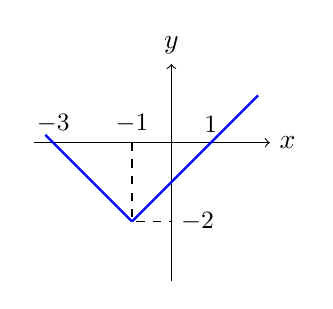
\begin{tikzpicture}[scale=0.5]
            % Eixos
            \draw[->] (-3.5,0) -- (2.5,0) node[right] {\(x\)};
            \draw[->] (0,-3.5) -- (0,2) node[above] {\(y\)};

            % Gráfico da função f(x) = |x+1| - 2
            \draw[domain=-3.2:-1, thick, blue] plot (\x, {- (\x + 1) - 2}); % x < -1
            \draw[domain=-1:2.2, thick, blue] plot (\x, {(\x + 1) - 2});    % x ≥ -1

            % Marcações das raízes (x = -3 e x = 1)
            \node[above] at (-3,0) {\small\(-3\)};
            \node[above] at (1,0) {\small\(1\)};

            % Marcação do vértice (x = -1)
            \draw[dashed] (-1,0) -- (-1,-2) -- (0,-2);
            \node[above] at (-1,0) {\small\(-1\)};
            \node[right] at (0,-2) {\small\(-2\)};
        \end{tikzpicture}
        &
        (b) 
        &
        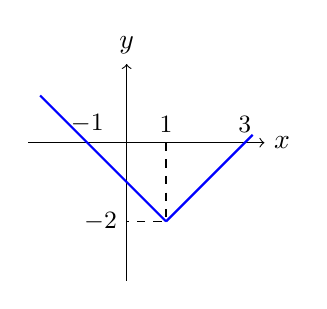
\begin{tikzpicture}[scale=0.5]
            % Eixos
            \draw[->] (-2.5,0) -- (3.5,0) node[right] {\(x\)};
            \draw[->] (0,-3.5) -- (0,2) node[above] {\(y\)};

            % Gráfico da função f(x) = |x+1| - 2
            \draw[domain=-2.2:1, thick, blue] plot (\x, {- (\x - 1) - 2}); % x < -1
            \draw[domain=1:3.2, thick, blue] plot (\x, {(\x - 1) - 2});    % x ≥ -1

            % Marcações das raízes (x = -3 e x = 1)
            \node[above] at (3,0) {\small\(3\)};
            \node[above] at (-1,0) {\small\(-1\)};

            % Marcação do vértice (x = -1)
            \draw[dashed] (1,0) -- (1,-2) -- (0,-2);
            \node[above] at (1,0) {\small\(1\)};
            \node[left] at (0,-2) {\small\(-2\)};
        \end{tikzpicture}
        &
        (c)
        &
        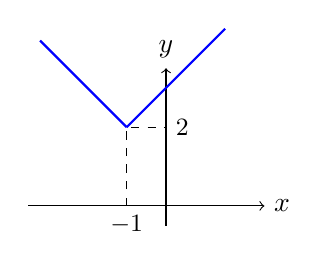
\begin{tikzpicture}[scale=0.5]
            % Eixos
            \draw[->] (-3.5,0) -- (2.5,0) node[right] {\(x\)};
            \draw[->] (0,-0.5) -- (0,3.5) node[above] {\(y\)};

            % Gráfico da função f(x) = |x+1| - 2
            \draw[domain=-3.2:-1, thick, blue] plot (\x, {- (\x + 1) + 2}); % x < -1
            \draw[domain=-1:1.5, thick, blue] plot (\x, {(\x + 1) + 2});    % x ≥ -1

            % Marcações das raízes (x = -3 e x = 1)
            %\node[below] at (-3,0) {\small\(-3\)};
            %\node[below] at (1,0) {\small\(1\)};

            % Marcação do vértice (x = -1)
            \draw[dashed] (-1,0) -- (-1,2) -- (0,2);
            \node[below] at (-1,0) {\small\(-1\)};
            \node[right] at (0,2) {\small\(2\)};
        \end{tikzpicture}
        \\
        (d)
        &
        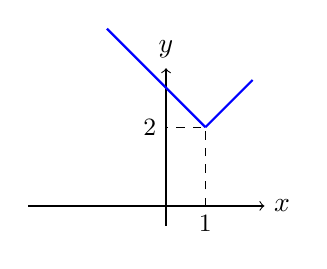
\begin{tikzpicture}[scale=0.5]
            % Eixos
            \draw[->] (-3.5,0) -- (2.5,0) node[right] {\(x\)};
            \draw[->] (0,-0.5) -- (0,3.5) node[above] {\(y\)};

            % Gráfico da função f(x) = |x+1| - 2
            \draw[domain=-1.5:1, thick, blue] plot (\x, {- (\x - 1) + 2}); % x < -1
            \draw[domain=1:2.2, thick, blue] plot (\x, {(\x - 1) + 2});    % x ≥ -1

            % Marcações das raízes (x = -3 e x = 1)
            %\node[above] at (3,0) {\small\(3\)};
            %\node[above] at (-1,0) {\small\(-1\)};

            % Marcação do vértice (x = -1)
            \draw[dashed] (1,0) -- (1,2) -- (0,2);
            \node[below] at (1,0) {\small\(1\)};
            \node[left] at (0,2) {\small\(2\)};
        \end{tikzpicture}
        &
        (e) 
        &
        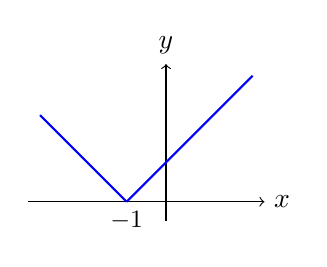
\begin{tikzpicture}[scale=0.5]
            % Eixos
            \draw[->] (-3.5,0) -- (2.5,0) node[right] {\(x\)};
            \draw[->] (0,-0.5) -- (0,3.5) node[above] {\(y\)};

            % Gráfico da função f(x) = |x+1| - 2
            \draw[domain=-3.2:-1, thick, blue] plot (\x, {- (\x + 1)}); % x < -1
            \draw[domain=-1:2.2, thick, blue] plot (\x, {(\x + 1)});    % x ≥ -1

            % Marcações das raízes (x = -3 e x = 1)
            %\node[above] at (-3,0) {\small\(-3\)};
            \node[below] at (-1,0) {\small\(-1\)};

            % Marcação do vértice (x = -1)
            %\draw[dashed] (-1,0) -- (-1,-2) -- (0,-2);
            %\node[above] at (-1,0) {\small\(-1\)};
            %\node[right] at (0,-2) {\small\(-2\)};
        \end{tikzpicture}
        &&
    \end{tabular}
\end{center}
%
}

% Define a resposta correta
\newcommand{\resposta}{D}

% Lógica condicional para exibição
\ifdefstring{\atividade}{lista}{%
    \alternativas
    \vspace{0.5em}
    
    \noindent\textbf{Resposta:} letra \textbf{\resposta}.
}{%
    \ifdefstring{\modo}{objetivo}{%
        \alternativas
    }{%
        % modo = discursiva → não mostra alternativas
    }
}
\end{exercicioBanco}

